\documentclass[12pt,a4paper]{article}\usepackage[]{graphicx}\usepackage[]{color}
%% maxwidth is the original width if it is less than linewidth
%% otherwise use linewidth (to make sure the graphics do not exceed the margin)
\makeatletter
\def\maxwidth{ %
  \ifdim\Gin@nat@width>\linewidth
    \linewidth
  \else
    \Gin@nat@width
  \fi
}
\makeatother

\definecolor{fgcolor}{rgb}{0.345, 0.345, 0.345}
\newcommand{\hlnum}[1]{\textcolor[rgb]{0.686,0.059,0.569}{#1}}%
\newcommand{\hlstr}[1]{\textcolor[rgb]{0.192,0.494,0.8}{#1}}%
\newcommand{\hlcom}[1]{\textcolor[rgb]{0.678,0.584,0.686}{\textit{#1}}}%
\newcommand{\hlopt}[1]{\textcolor[rgb]{0,0,0}{#1}}%
\newcommand{\hlstd}[1]{\textcolor[rgb]{0.345,0.345,0.345}{#1}}%
\newcommand{\hlkwa}[1]{\textcolor[rgb]{0.161,0.373,0.58}{\textbf{#1}}}%
\newcommand{\hlkwb}[1]{\textcolor[rgb]{0.69,0.353,0.396}{#1}}%
\newcommand{\hlkwc}[1]{\textcolor[rgb]{0.333,0.667,0.333}{#1}}%
\newcommand{\hlkwd}[1]{\textcolor[rgb]{0.737,0.353,0.396}{\textbf{#1}}}%
\let\hlipl\hlkwb

\usepackage{framed}
\makeatletter
\newenvironment{kframe}{%
 \def\at@end@of@kframe{}%
 \ifinner\ifhmode%
  \def\at@end@of@kframe{\end{minipage}}%
  \begin{minipage}{\columnwidth}%
 \fi\fi%
 \def\FrameCommand##1{\hskip\@totalleftmargin \hskip-\fboxsep
 \colorbox{shadecolor}{##1}\hskip-\fboxsep
     % There is no \\@totalrightmargin, so:
     \hskip-\linewidth \hskip-\@totalleftmargin \hskip\columnwidth}%
 \MakeFramed {\advance\hsize-\width
   \@totalleftmargin\z@ \linewidth\hsize
   \@setminipage}}%
 {\par\unskip\endMakeFramed%
 \at@end@of@kframe}
\makeatother

\definecolor{shadecolor}{rgb}{.97, .97, .97}
\definecolor{messagecolor}{rgb}{0, 0, 0}
\definecolor{warningcolor}{rgb}{1, 0, 1}
\definecolor{errorcolor}{rgb}{1, 0, 0}
\newenvironment{knitrout}{}{} % an empty environment to be redefined in TeX

\usepackage{alltt}

\usepackage{times}
\usepackage{durhampaper}

\usepackage{booktabs}
\usepackage[table]{xcolor}
\usepackage{tikz}
\usepackage{lastpage}%page 1 of \lastpage
\usepackage{float}
\usepackage{flafter}
\usepackage[british]{babel}%hypenation and spelling and stuff
\usepackage{fancyhdr}
\usepackage{subcaption}
\usepackage[section]{placeins}
\usepackage{natbib}

%packages to load last
\usepackage[hyphens, spaces]{url}%allow URLS
\usepackage{varioref}%Automatic page references
\usepackage[colorlinks, allcolors=blue, breaklinks]{hyperref}%Automatic reference links
\usepackage[all]{hypcap}
\usepackage[capitalise, nameinlink]{cleveref}%Automatic reference typing

\renewcommand{\harvardurl}[1]{\textbf{URL:} \url{#1}}
%\citationmode{abbr}
\bibliographystyle{agsm}

\title{Tailoring Horror Games with Biometrics}
\author{} % leave; your name goes into \student{}
\student{S.H. Lowes}
\supervisor{M.J.R. Bordewich}
\degree{BSc Computer Science}

\date{}


\pagestyle{fancy}
\pagenumbering{arabic}
\rhead{\small Steven Lowes}

\makeatletter
\lhead{\small \@title}
\makeatother

\lfoot{3rd May 2019}
\cfoot{Page \thepage\ of \pageref{LastPage}}
\begin{document}





\maketitle

\begin{abstract}
%These instructions give you guidelines for preparing the final paper.  DO NOT change any settings, such as margins and font sizes.  Just use this as a template and modify the contents into your final paper.  Do not cite references in the abstract.

%The abstract must be a Structured Abstract with the headings {\bf Context/Background}, {\bf Aims}, {\bf Method}, {\bf Results}, and {\bf Conclusions}.  This section should not be longer than half of a page, and having no more than one or two sentences under each heading is advised.

\textbf{Context/Background}

\textbf{Aims}

\textbf{Method}

\textbf{Results}


\end{abstract}

\begin{keywords}
Put a few keywords here.
\end{keywords}

\section{Introduction}
%This section briefly introduces the general project background, the research question you are addressing, and the project objectives.  It should be between 2 to 3 pages in length.  Do not change the font sizes or line spacing in order to put in more text.

%Note that the whole report, including the references, should not be longer than 20 pages in length.  The system will not accept any report longer than 20 pages.  It should be noted that not all the details of the work carried out in the project can be represented in 20 pages.  It is therefore vital that the Project Log book be kept up to date as this will be used as supplementary material when the project paper is marked.  There should be between 10 and 20 referenced papers---references to Web based pages should be less than 10\%.

This study will explore whether users show any preference between a horror game where jump scares are randomly allocated and the same game where jump scares are tailored based on biometric feedback. An extensive user study will be conducted and the results analysed to explore the difference in self-reported user enjoyment and data gathered from biometrics measuring how scared the users were.

This work could act as a launching point for other games integrating the use of sensors. With smartwatches becoming increasingly ubiquitous, in the future many games could access the sensors in those smartwatches to adjust gameplay. Sensor-enabled gameplay adjustment could be applied to other forms of entertainment. For example, action games could integrate biometrics by enabling slow-motion after detecting high-adrenaline moments. Games could further integrate biometrics as a central mechanic, i.e. in order to continue through the game you must learn to control your body's semi-autonomous responses. This tight integration of biometrics would allow for a new paradigm in computer entertainment.

Ultimately, this work aims to validate that the use of biometrics can lead to an improved gameplay experience, utilising horror games as the most ideal scenario during this exploratory phase.

\subsection{Prior Work}
The original plan for this project was to explore the use of EDA to find relaxing music. By representing songs as 14-dimensional vectors, where each component of the vector was a high-level quality of the song such as `acousticness' or `danceability', the problem could be treated as an AI search problem. Each song can be assigned a fitness based on how relaxing a user finds it when listening to it. The problem becomes to simply explore the 14-dimensional space of all songs and find the song with highest fitness.

However, there were two problems which meant that this project was entirely infeasible. Firstly, calculating the fitness of a song took the length of the song to do, since a human needed to listen to the song. To find a near-optimal solution in the dataset of 25 million songs that was used would take thousands of songs, which would mean weeks of music listening.

Secondly, it was discovered that the EDA sensor was a poor choice for the task of measuring how relaxing music was. For many of the reasons that EDA is a great choice for horror games, it is a terrible choice for music. There is no single stimulus that can be measured, meaning that it's impossible to decide whether a change in EDA was caused by the music or, for example, the user seeing a bird out of the window. In addition to this, EDA tends to drift over time, causing measurements to be thrown off by the temperature of the room and how hungry the user was. When working with a single stimulus, such as in horror games, the recording length is not long enough for this to cause an issue.

\section{Related Work}
%This section presents a survey of existing work on the problems that this project addresses.  it should be between 2 to 4 pages in length.  The rest of this section shows the formats of subsections as well as some general formatting information for tables, figures, references and equations.

\subsection{EDA}
Physiological arousal is a measure of how alert the body is. It can be caused by intense emotion, shock, or surprise, and is strongly linked to the `fight or flight' reflex. When experiencing high arousal, the body's blood pressure and heart rate increases, readying the body to respond to a stimulus \citet[pp.162-167]{arousal}.

When the body is becoming more aroused, it leads to an increase in `Electrodermal Activity' (EDA). EDA is a measure of how much the body is sweating, and is measured by testing the resistance between two electrodes. When the participant experiences high EDA, the resistance between the electrodes decreases \citet[pp.2-3]{eda}. GSR (galvanic skin response) is a synonymous (though outdated) term for EDA, which is notably used in the name of the EDA sensor that the system uses.

EDA is used in many applications, including as part of the polygraph (lie-detector) test, where it can detect the physiological arousal caused by lying and being afraid of the repercussions of doing so \citet{polygraph}. It is also used by the `Church of Scientology' to guide therapy in removing any negative associations from words and concepts, a controversial technique known as `auditing' \citet[p.32]{auditing}.

The EDA response consists of a sharp drop in resistance, over a period of {\raise.17ex\hbox{$\scriptstyle\sim$}}1s, when arousal passes a certain threshold (the size of the drop correlates with the extent of the arousal), followed by an asymptotic increase in resistance back to a high base value, with a half-life of {\raise.17ex\hbox{$\scriptstyle\sim$}}10s. The initial drop occurs 1-3 seconds after the stimulus. That high base value is rarely reached because arousal varies frequently even without any explicit stimulus, so the EDA response happens quite often \citet{edaAnalysis}.

\subsection{Biometrics}
Biometrics are becoming increasingly ubiquitous. 67\% of smartphones include a fingerprint scanner \citet{fingerprint}, and 141 million smartwatches were sold in 2018 \citet{smartwatches}, nearly all of which are constantly taking heart-rate measurements.

Consumers are increasingly becoming accustomed to the fact that wearable tech and biometrics can be used to improve their user experience. Despite this, biometrics have seen little use in the entertainment industry.

As biometrics become more accepted and more integrated, they will allow for a new step in human-computer interfacing. Just as the inclusion of a fingerprint sensor allowed smartphones to identify their user autonomously, integrated sensors will allow applications to get immediate feedback without the user having to switch contexts and give a rating. This means that they can iteratively improve without user or developer intervention. Eventually, these biometrics will extend to the point of brain-computer interfacing, where the program can adjust to the individual tastes and preferences of the user without having to test the available options individually.

\subsection{Horror Games}
The horror games industry is huge, with over 2000 unique titles on steam and almost 500 million copies owned \citet{horrorSteamSpy}. The vast majority of these games present the same experience to all players, though there have been experiments in tailoring the games to the individual. Games such as  \emph{Nevermind} \citet{nevermind}, and \emph{Bring to Light} \citet{bringtolight} both allow the use of heart-rate monitors to adjust gameplay.

The use of heart rate monitors in these games is not ideal, but makes sense for a mass-market game as heart rate sensors are some of the most widely available biometric sensors. Heart rate sensors are limited as they struggle to show the immediate response to a scare. They can tell how scared a person is, but not how scared an individual event made them. In contrast, this project will use EDA sensors which can detect changes on the order of milliseconds, making them an ideal feedback mechanism in a horror game \citet{edaAnalysis}.

Horror games are perfect for measuring with biometrics, as we have a defined event which we know will cause a large reaction, and we can use the sensors to measure the response to that known event. This is similar to with a lie detector - we have an event (a person answering a question) and we want to see whether it caused a response. This is much simpler than trying to detect stress over a long period as the timing of the known stimulus can be used to predict a change in biometrics.

\section{Solution}

\subsection{Algorithm}

\begin{figure}[htb]


{\centering \includegraphics[width=\maxwidth]{figure/ExampleEda-1} 

}



\caption{One participant's recorded EDA data}
\label{fig:ExampleEda}
\end{figure}

\begin{figure}[htb]


{\centering 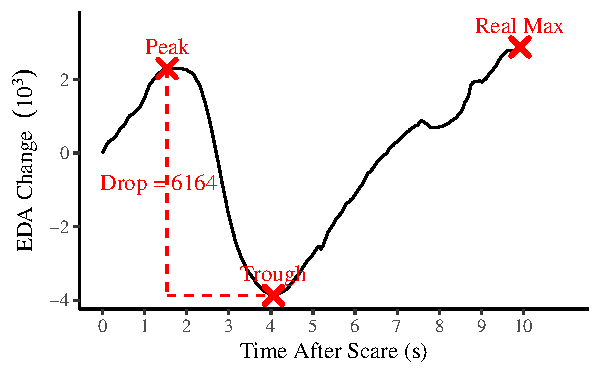
\includegraphics[width=\maxwidth]{figure/ExampleScare-1} 

}



\caption{How the drop value is calculated}
\label{fig:ExampleScare}
\end{figure}

Based on preliminary testing and experimentation, an algorithm was devised.
The algorithm adjusts the timing of jump scares in a horror game.
It aims to prevent users from becoming desensitized to them, by lengthening the delay between scares when the user is not reacting as greatly as they were previously. It shortens the delays when they react more strongly.
Since everyone reacts differently to the jump scares, we can't just say x number of points = very scared, x - delta = less scared.
People with higher EDA will drop more and some people are more easily scared than others.
Therefore instead of doing that we use the first 3 scares to calibrate the algorithm.
It does not kick in until after the 3rd scare.
The first 4 scares happen with delays of 20-30 seconds between them
It works as follows:
Look at all previous scares, and compute the drop. The drop is computer by finding the minimum EDA value seen in the 10 seconds after the scare occurs (the trough).
Then, find the highest EDA value seen between the scare and the trough (the peak). The absolute difference in EDA between the peak and the trough is the drop.
Looking at the list of all previous drops seen, compute the mean and standard deviation. Then, 10s after each future scare, compute the drop for that scare. Figure out how many standard deviations above/below the mean that it was, and adjust as follows:

\begin{equation}
d_{n+1} = d_n * \exp^{-0.366 * \frac{s_n - \mu}{\sigma}}
\end{equation}

where $d$ is the delay between scares, $s$ is the size of the drop, $\mu$ is the mean size of all previous drops, and $\sigma$ is the standard deviation in the size of all previous drops. 

An arduino uno was used to read from the EDA sensor.
It is programmed to sit in a loop, repeatedly reading the EDA sensor.
To reduce the noise in the data and to reduce the volume of data recorded, it takes 10 readings and sums them, then reports the sum value. This still results in frequent data - one reading every 5-10 ms.

The horror game itself was created as a minecraft mod.
This allowed the game to be created with far less effort, using minecraft as a game engine and its mature open-source modding API, forge, to create my game.
Originally, i was concerned about the difficulty of creating a game scary enough that we would be able to get a measurable response from the sensor.
However, the sensor is incredibly sensitive.
Even jump scares which the user knew were coming, and was just a static screen saying "boo" was enough to get a response.
This meant that the final jump scare, a scary monster face and loud noise, generated a suitably large effect that could easily be measured and analysed.

A `creeper' face appears large on the screen, taking up most of the user's field of view. The creeper is a monster in Minecraft and has a reasonably scary appearance. At the same time, a loud noise plays. The noise consists of many in-game noises pitch-shifted and played at the same time. It is has many low frequencies and some high-pitched scream-like sounds. See \vref{fig:JumpScare}.

\begin{figure}[htb]
	\centering
	
\includegraphics[width=0.5\linewidth]{images/scare.png}
	\caption{The Jump Scare}
	\label{fig:JumpScare}
\end{figure}


Players were given a task to complete in the game - to explore a haunted house for 10 minutes, searching for 16 coloured wool in hidden chests.
This was done to increase the tension felt by the players, as they could easily sit in a corner without moving.
The game was set in a haunted house with spooky music playing. The environment and music are the same in all playtests.

There was no way for players to die, as any implementation where the jump-scare poses a threat necessarily means that good timing of the jump scare requires environmental knowledge.
The only knowledge the algorithm has is the previous responses, therefore it must be possible to correctly time the jump scares with only that knowledge - otherwise we'll never see good results.

After 10 minutes, the players are informed that the game is complete and the jump scares stop.

Data from the sensor is recorded throughout the test.
Also, the direction that the player is facing in-game is recorded.
Exact timings of the scares are also recorded.
When the test ends, all of this data is saved to a JSON file, which can be passed to the algorithm for the control group - in which case it just replicates the scare timings.

\subsection{Implementation}

\begin{figure}[!htbp]
	\centering
	\begin{tikzpicture}
	\draw  [thick](-0.5,0.5) rectangle (-3,-0.5);
	\node at (-1.75,0) {Arduino Uno};
	\node (v6) at (-1.75,0.5) {};
	\node at (-1.75,1.5) {EDA Sensor};
	\draw  [thick](-3.5,-1.5) rectangle (0,-5.5);
	\node (v8) at (-3,0) {};
	\node (v7) at (-3.5,-2) {};
	\node (v4) at (-5,0) {};
	\node (v5) at (-5,-2) {};
	\draw  (v4) edge (v5);
	\draw  [->] (v5) edge (v7);
	\draw  (v8) edge (v4);
	\node at (-4,0.25) {USB Cable};
	\draw  (-3.5,-1.5) rectangle (0,-2.5);
	\node at (-1.75,-2) {jrxtx};
	\node at (-1.75,-1.25) {Minecraft};
	\node (v9) at (-1.75,-5) {Wait};
	\node (v10) at (-2.75,-3.5) {Trigger};
	\node (v11) at (-0.75,-3.5) {Measure};
	\node (v12) at (-2.75,-2.5) {};
	\node (v13) at (-0.75,-2.5) {};
	\draw [->] (v10) edge (v12);
	\draw [->] (v13) edge (v11);
	\draw [->] (v11) edge (v9);
	\draw [->] (v9) edge (v10);
	\draw [->] (v10) edge (v11);
	\node at (-4.25,-1.75) {Serial};
	\draw [->] (-1.75,1.5) node (v1) {} circle (0.5);
	\draw [->] (v1) edge (v6);
	\end{tikzpicture}
	\caption{Hardware + Software Architecture}
\end{figure}

\section{Experimental Study}

An experimental study was performed.
The null hypothesis is: Using the algorithm to tailor jump scare timings shows no difference in results compared to using a pre-determined set of timings.

Participants were put into one of two groups.
The intervention group played the game with the algorithm running.
The control group played the game with the jump scare timings pre-determined before they started playing.

There were lots of controls outside of what was mentioned in the previous section:
Controlling for scaredness - each participant was asked.
Each participant was paired with someone in the other group that gave the same answer.
This means that both the intervention and control groups show the same distribution of answers to this question, seen in the figure below.
This is stratified sampling.

\begin{figure}[htb]


{\centering 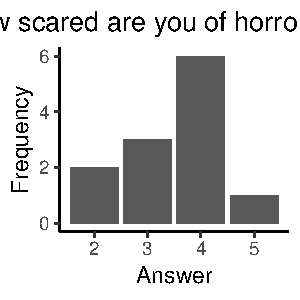
\includegraphics[width=\maxwidth]{figure/ParticipantScaredness-1} 

}



\caption{The distribution of how scared each group is of horror games/films in general}
\label{fig:ParticipantScaredness}
\end{figure}

To control for the number of scares (so we have the same distribution of number of scares in both groups) - we run the intervention group first because the algorithm doesn't support targeting a number of scares - it depends on how the person reacts.
Then, we run the control group tests. Each person on the control group was shown the same number of scares as the person they were paired with in the previous control.

\begin{figure}[htb]


{\centering 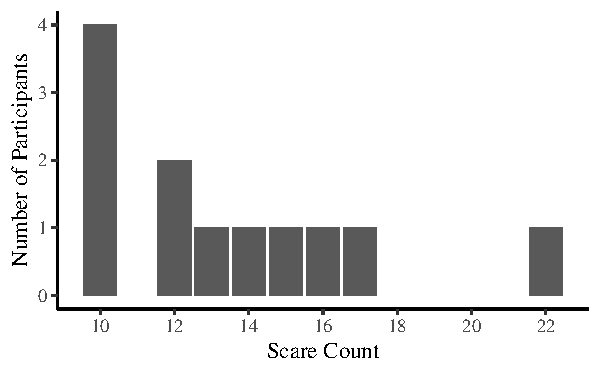
\includegraphics[width=\maxwidth]{figure/ParticipantScares-1} 

}



\caption{Each group's distribution of the number of times a participant was scared}
\label{fig:ParticipantScares}
\end{figure}

To control for the timing of scares - the pre-determined timings for the control group were just the timings of their intervention-group partner.
This means that for each pair that was paired up in that first control, they were shown the same number of scares at exactly the same timings, the difference being that the timings were based on the intervention-group participant's response, and not the control group participants.

Some threats to the validity of the study were present:

Firstly, the majority of the participants were young, male, and many of them were computer scientists.
I did not collect demographic data, to protect the anonymity of my participants, therefore don't have hard number, but the categories male, 18-25, and computer scientist were all in the majority.
Also, the experimental setting changed frequently.
Some tests were performed in the computer science department, which contains many other people and many distractions, while other tests were performed in quiet, private areas.
Additionally, some tests were performed at social events, meaning that participants had been drinking alcohol - though no participant was noticeably drunk.
These factors were not recorded and therefore we cannot investigate any correlation between the environmental/demographic factors and results.
While I don't believe that these threats completely invalidate the study, it does mean that any marginal results should be used only to direct further research as opposed to being taken as gospel.

I originally aimed to get 50 participants. Due to practical issues, only 26 participants were tested. Of those, 2 participants were excluded from analysis as their EDA went too low and the sensor stopped working. Of the remaining 24 participants, 12 were allocated to each group. After 21 participants, Easter break was arriving and people would start to leave Durham, so I wouldn't be able to test more. At that point I started looking only for people to be the control-group participant in the pairs that only had intervention group participants. I was careful not to let people know what number they had to say to the scaredness question to be accepted.

Ethics:
Consent was gathered and participants were asked to sign consent forms.
Harm was prevented by allowing participants to ask questions, see the jump-scare, and drop out freely.
Confidentiality was achieved by using participant IDs and only linking ID to name in the consent forms, which were securely destroyed after the experiment was done. Data was stored on a password-protected device and only released if the participants signed the voluntary data release (which all participants did).
Equipoise - it's uncertain whether the intervention would be effective or better/worse, and even if it is effective it's not obvious that a scarier game is better/worse.

\section{Results}

First we will examine the results of the questions asked to participants after their playtest was completed, before moving on to analyse the raw data from the sensor.

Participants were asked how much they enjoyed their time playing the game.
The answers given by each group are presented in \vref{fig:ParticipantEnjoyment}.
In general, participants in the intervention group enjoyed the game less than those in the control group.

\begin{figure}
  \centering
  \begin{subfigure}[t]{.49\linewidth}


{\centering 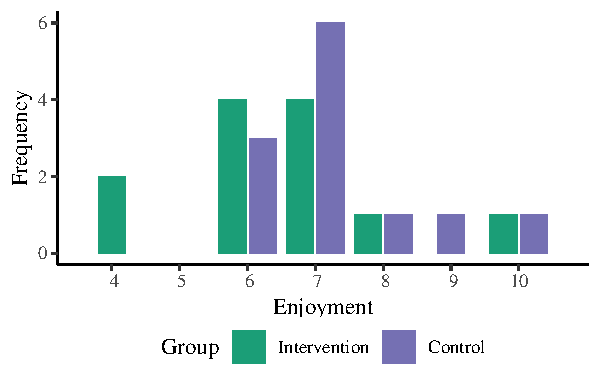
\includegraphics[width=\maxwidth]{figure/ParticipantEnjoyment-1} 

}



  	\caption{Distribution of Responses}
  \end{subfigure}
  \begin{subfigure}[t]{.49\linewidth}


{\centering 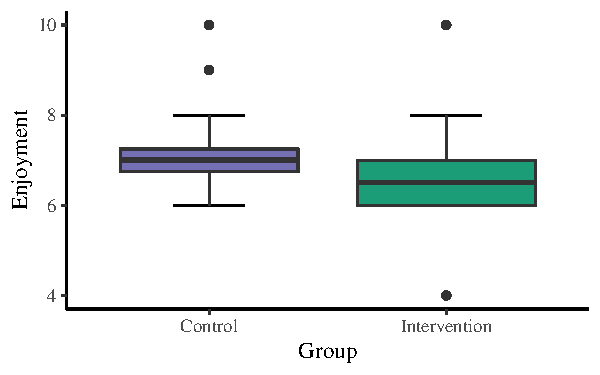
\includegraphics[width=\maxwidth]{figure/ParticipantEnjoymentBoxPlot-1} 

}



  	\caption{Comparison between Groups}
  \end{subfigure}
  \caption{On a scale of 1-10, how much did you enjoy that as a game?}
  \label{fig:ParticipantEnjoyment}
\end{figure}

Participants were asked to rate the frequency of the jump scares from "Far Too Few" to "Far Too Many" jump scares.
The answers given by each group are presented in \vref{fig:ParticipantTiming}.
Most participants felt there were too many jump scares.
Their feeling is backed up by the scare timing histogram in \vref{fig:ScareHistogram}.
Generally, the algorithm decreased the frequency of jump scares over time.

The control group felt marginally more strongly that there were too many scares.
Since the two groups had identical scare timings, this was not the result of any difference in the real frequency between the groups.
Therefore, this suggests that the scares were badly timed for the control group, making them more aware of the scares and making the scares less immersive.

Graph B in \cref{fig:ParticipantTiming} shows a statistically significant correlation between the real frequency of scares and the participants' perceived scare frequency.
This indicates that participants are accurately assessing the frequency of jump scares and that we are not just seeing trends in random data.

\begin{figure}
  \centering
  \begin{subfigure}[t]{.49\linewidth}


{\centering 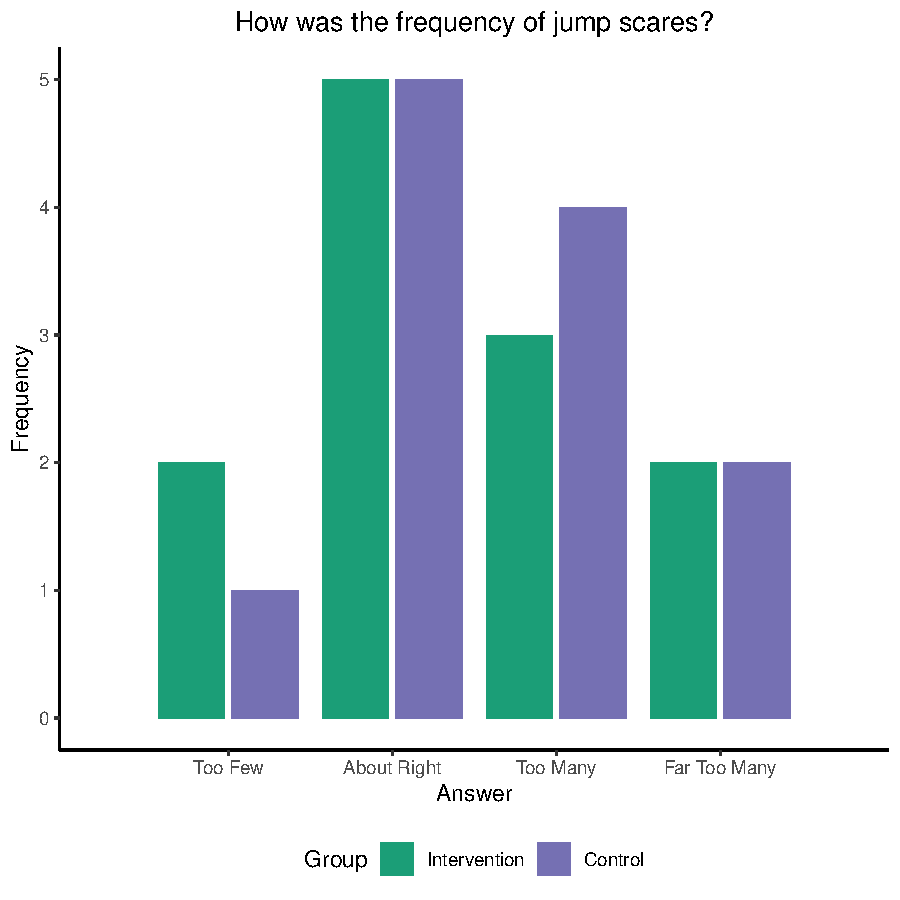
\includegraphics[width=\maxwidth]{figure/ParticipantTiming-1} 

}



		\caption{Distribution of Responses}
  \end{subfigure}
  \begin{subfigure}[t]{.49\linewidth}


{\centering 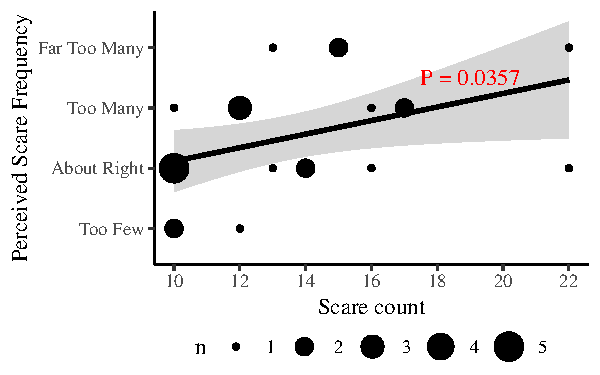
\includegraphics[width=\maxwidth]{figure/ScareFrequency-1} 

}



  	\caption{Actual vs Perceived frequency}
  \end{subfigure}
  \caption{How was the frequency of jump scares?}
  \label{fig:ParticipantTiming}
\end{figure}

\begin{figure}[htb]


{\centering 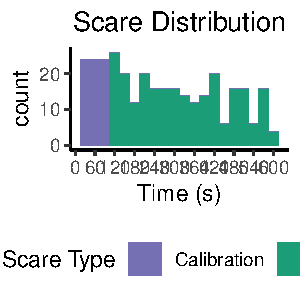
\includegraphics[width=\maxwidth]{figure/ScareHistogram-1} 

}



\caption{Scare Frequency over Time}
\label{fig:ScareHistogram}
\end{figure}

We will now discuss the data recorded from the EDA sensor.
The raw data from the sensor is shown in \vref{fig:RawData}.
This has already been normalised so that the playtest starts at $x=0$.
The actual data records wallclock time for each measurement as well as wallclock time for when the playtest starts, which we used to normalise the data.

This data requires significant cleanup before it is ready to be analysed.
The data was recorded in full so that the relevant parts could be extracted during analysis --- so as to not make any analysis decisions pre-emptively.

\begin{figure}[htb]


{\centering 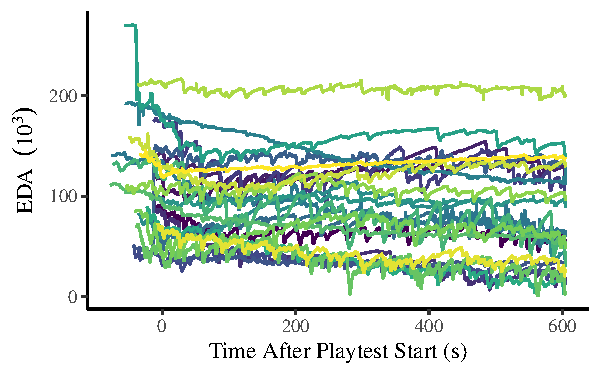
\includegraphics[width=\maxwidth]{figure/RawData-1} 

}



\caption{The raw data from the sensor}
\label{fig:RawData}
\end{figure}

The drop is calculated using the 10 seconds after each scare.
\vref{fig:PerGroupScares} shows the data after filtering to just the 10 seconds after each scare and colouring the lines based on which group the participant is in.
Lines with a larger vertical drop generally indicate a person that was more scared by the jump-scare.

\begin{figure}[htb]


{\centering 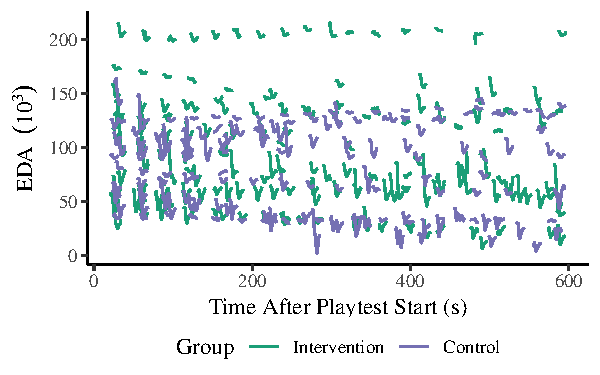
\includegraphics[width=\maxwidth]{figure/PerGroupScares-1} 

}



\caption{The scare data, coloured per group}
\label{fig:PerGroupScares}
\end{figure}

By normalising all of these scares to start at $x,y = 0$, and taking the mean of each group's lines, we can see each group's average scare.
We can also calculate a standard error margin around these means.
When doing this, we filter out the first 3 scares for each participant as the algorithm hasn't kicked in so they're essentially both control groups.
\vref{fig:ResponseAfterScare} shows the average scare for each group and the difference between the two groups.
The two groups are significantly different, with participants in the intervention group seeing their EDA fall for longer and to a lower trough value.
The intervention group also takes longer to recover, with the two lines still being separated by more than the margin of error after 10 seconds.
Additionally, the intervention group reacts slightly quicker than the control group, with the EDA starting to drop slightly earlier than it does for the control group.

\begin{figure}
  \centering
  \begin{subfigure}[t]{.49\linewidth}


{\centering 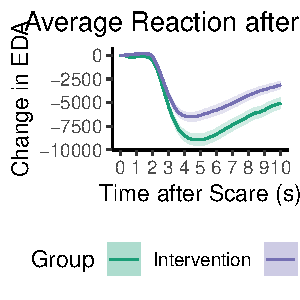
\includegraphics[width=\maxwidth]{figure/ResponseAfterScare-1} 

}



    \caption{Per-Group Average}
  \end{subfigure}
  \begin{subfigure}[t]{.49\linewidth}


{\centering 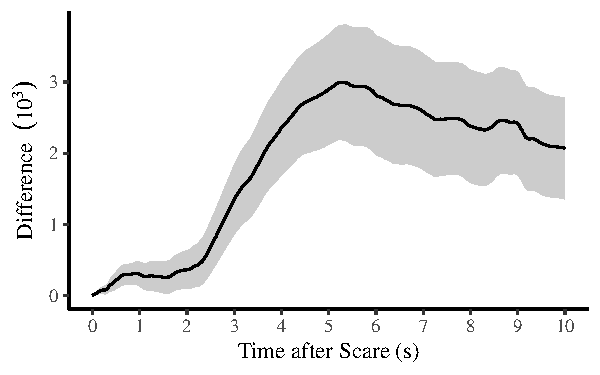
\includegraphics[width=\maxwidth]{figure/CompareGroups-1} 

}



    \caption{Difference between Groups}
  \end{subfigure}
  \caption{Average Response to a Jump-Scare}
  \label{fig:ResponseAfterScare}
\end{figure}

\begin{figure}
	\centering
	\begin{subfigure}[t]{.49\linewidth}


{\centering 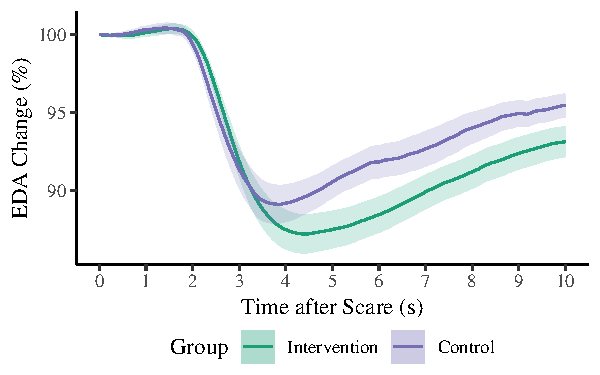
\includegraphics[width=\maxwidth]{figure/ResponseAfterScareRel-1} 

}



		\caption{Per-Group Average}
	\end{subfigure}
	\begin{subfigure}[t]{.49\linewidth}


{\centering 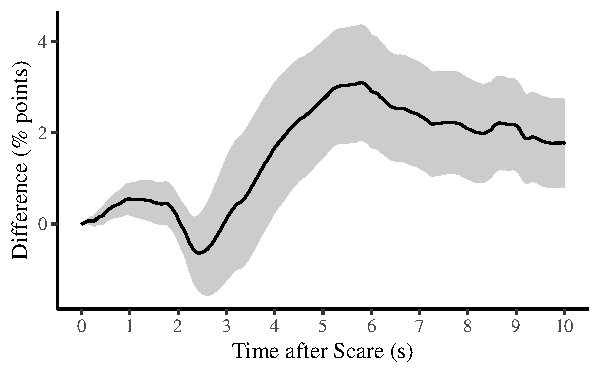
\includegraphics[width=\maxwidth]{figure/CompareGroupsRel-1} 

}



		\caption{Difference between Groups}
	\end{subfigure}
	\caption{Average Relative Response to a Jump-Scare}
	\label{fig:ResponseAfterScareRel}
\end{figure}

If we take the data from \vref{fig:PerGroupScares}, and convert each scare line to its calculated drop value, we can plot how the size of the drop changes over time.
\vref{fig:ScarednessOverTime} shows every scare that occurred during the experiments, and plots one linear regression per group.
At the time of the first scares, the linear regressions predict almost exactly the same scaredness between the two groups.
This is a strong indication that the sample is valid and that the two groups begin with the same reactions before the algorithm has kicked in.
As time goes on, the linear regressions diverge, separating by more than a 95\% confidence interval by the mid-way point of the play test.
This indicates that the timing algorithm prevents the intervention group from becoming bored by the jump-scares, while the control group does become bored without it.

\vref{tab:RegressionTable} shows the relevant statistics of the two regressions.
The P-Value of the control group is under 0.01, and its gradient is negative, indicating a statistically significant trend.
Over time, the control group becomes less scared of the jump-scares.
The R-Squared value indicates that around 4\% of a control-group participant's response to a scare can be predicted solely by how long they have been playing.
The gradient indicates that for each second played, a participant in the control group would respond to a scare with a drop that is 8.5 points smaller.

In comparison, the P-Value of the intervention group is above 50\%, indicating that it's likely there is no correlation between time played and scaredness in the intervention group.
Even if there was a correlation, the gradient is positive indicating that participants actually become more scared over time.

\begin{figure}
  \centering
  \begin{subfigure}[t]{.49\linewidth}


{\centering 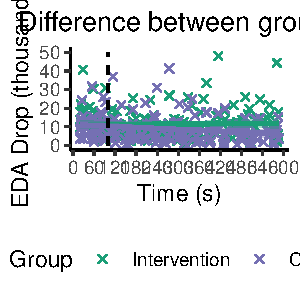
\includegraphics[width=\maxwidth]{figure/ScarednessOverTime-1} 

}



    \caption{All data}
  \end{subfigure}
  \begin{subfigure}[t]{.49\linewidth}


{\centering 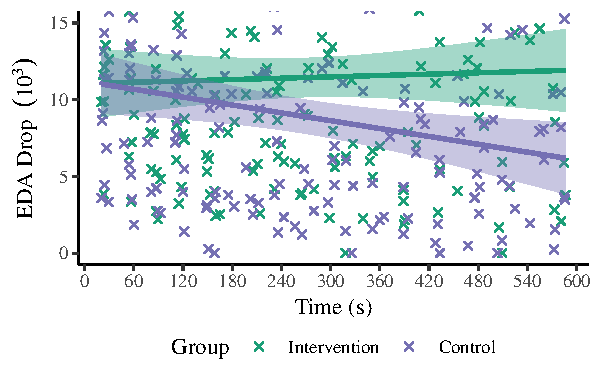
\includegraphics[width=\maxwidth]{figure/ScarednessOverTimeCrop-1} 

}



    \caption{Cropped}
  \end{subfigure}
  \caption{Scaredness over Time}
  \label{fig:ScarednessOverTime}
\end{figure}

\begin{table}[t]

\caption{\label{tab:RegressionTable}Relevant statistics for the Regressions}
\centering
\begin{tabular}{cccc}
\toprule
\textbf{Model} & \textbf{Gradient} & \textbf{R-Squared} & \textbf{P-Value}\\
\midrule
Intervention & 1.47 & 0.001 & 0.695\\
Control & -8.54 & 0.042 & 0.009\\
\bottomrule
\end{tabular}
\end{table}


\section{Evaluation}

\subsection{Threats to Validity}
I will analyse the threats to my study's validity using the framework %TODO thanks amie

\textbf{Attrition threat} - when the risk of people dropping out / being excluded is a function of the dependent variable. This risk is present in two ways. If people are very scared, their EDA will drop more (dependent variable), and those people will also be more likely to drop out. Therefore if one group is much scarier the result won't show as clearly as some will drop out over being too scared. This risk did not occur as nobody dropped out once starting. 2 people were excluded though, and they were excluded as a direct result of their EDA. If that was as a result of their EDA dropping a lot, that would be a risk. In our case, it was due to their natural EDA being very low, with one participant remarking even before any issues occurred that they had notoriously sweaty hands. I think the attrition threats are minimal.

\textbf{Maturation threat} - When the dependent variable is a function of time and there is a difference in time between the testing of the two groups. Since in each pair the intervention group participant is tested first, the intervention group tests on average happened before the control group tests. However, I doubt the dependent variable is a function of time - I don't think that people are any more or less scared of horror games from one week to the next and there were no newsworthy events that could have heightened people's sense of fear or anything like that.

The experiment was single-blind, in that I knew which group people were in but thy did not. There is limited researcher participation in the experiment so i doubt this has much of an effect. I just explained the test to them then set it going and everything happened passively.

The participants were not assigned to the groups randomly. They were assigned chronologically. As and when participants were available to be tested, they were asked for their scaredness and either placed in the control group and matched with an intervention group person or were placed int he intervention group and matched with a control group person later. Originally I planned to sample participants randomly by getting and initial expression of interest and a 1-5 scaredness rating then assigning groups and performing tests, but that was infeasible due to attrition rates and the general flakiness of students.

Other factors that could have had an effect and weren't controlled for:
Some people had played minecraft before, those that hadn't may have been more stressed. This was minimised by removing the chance of death, and giving detailed instructions and a constrained environment. The game was simple to learn and nobody showed any issues past the first 30 seconds or so.
Some people are more competitive when trying to collect the wool. This could have been stressful for them. This was not controlled for but there should not be any competitiveness bias between groups

There is a slim chance of intentional data vandalism. Participants could lie about how scared they were, but if we plot a scatter graph as in figure x, we don't see any clear evidence of lying. People generally follow the regression line, but with a wide variance. If there were 1 or 2 anomalies, that could suggest lying, but this just suggests that people are bad judges of how scared they are. Future tests could investigate better ways to control for scaredness. The P-value is not statistically significant so we can't say there is a relationship, but there's no evidence that this stratification is harmful, and some evidence that it is helpful.

\begin{figure}[htb]


{\centering 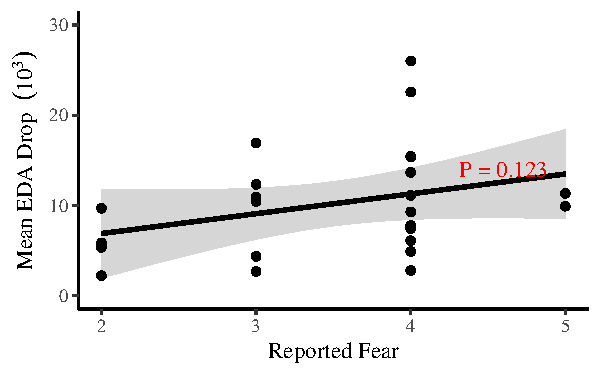
\includegraphics[width=\maxwidth]{figure/ReportedScaredness-1} 

}



	\caption{Drop size positively correlates with reported scaredness}
	\label{fig:ReportedScaredness}
\end{figure}

People have different EDA at the start of the playtest. Since you drop more with higher EDA, that's a problem and makes it hard to compare. There is a difference between groups in starting EDA.

\begin{figure}[htb]


{\centering 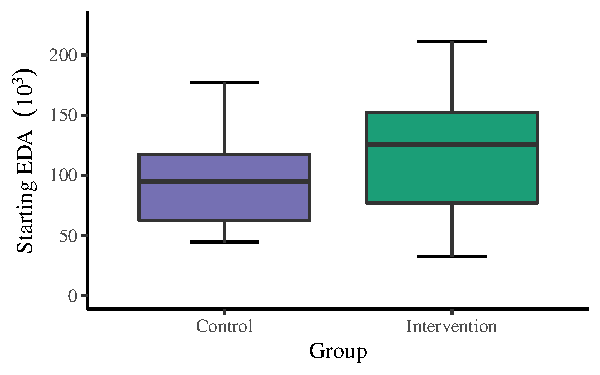
\includegraphics[width=\maxwidth]{figure/StartingEda-1} 

}



	\caption{The starting EDA for each group}
	\label{fig:StartingEda}
\end{figure}


People can train themselves to change their EDA at will, usually done to learn to beat a lie-detector test. That would be hard to detect, by design, but nobody showed any knowledge of EDA or GSR> It's hard to rule this out but it's a very niche skill and the chance of someone having that skill and intentionally vandalising the data is very slim.

Since the intervention group participants were in general found earlier than the control group participants, they are more likely to be closer to me as I started by asking my friends. That was pretty shit, but give me a break. Don't @ me. This probably has no effect.

Data is probably not generalisable to the population of all people - far too many threats. However, can be used to direct further study.
Not clear whether a 10-minute test would generalise to a multi-hour play session, but was forced to limit test length for practical reasons.
Not clear whether a simple game based in minecraft where all jump-scares are the same would generalise t o a more complex game, but needed to control as much about the scare as possible.

\subsection{Analysis}
There is a slight difference in participant enjoyment between groups, as seen in \vref{fig:ParticipantEnjoyment}.
Since it's a small difference, it could just be random due to the small sample size.
Or it could be due to biases in the sampling as discussed earlier.
Additionally, only one question about enjoyment was asked in the post-test questionnaire, and no demographic data was recorded, so we can't drill down to look into what could be causing a difference between groups.
Finally, the participants aren't the target audience for a horror game, as enjoying horror games wasn't a requirement to take part.
Further study to explore whether the algorithm improves enjoyment in horror-game players would be warranted.
It seems suspect that a horror game (that's not very scary to begin with) can become more scary but less enjoyable just by changing the timings.
Intuitively, those should be correlated.
This runs counter to intuition, which means it would be interesting to study further, but it's a small difference in a study with a small sample size, so it could easily just be random chance.
The use of a 10-point scale increases the effect of randomness.

There's a very marginal difference between groups when it comes to the perceived frequency of jump scares, as seen in \vref{fig:ParticipantTiming}.
It's fairly reassuring that the groups are so similar, seeing as they had the exact same timings, and that's what they were supposed to be rating.
This could be interesting to investigate further, and with a larger sample size you could say conclusively that there is a difference between groups.
If there is a difference between groups, this could be the beginning of further research into the perceived frequency of jump scares based on good vs bad timing.
As a purely theoretical excercise about the perception of horror games, there would be no requirement to use an algorithm.
You could just have a person manually trigger the jump scares at good times.
Would be interesting to control the number of jump scares but not the timing, then compare good vs bad timing and see how people rate the scare frequency.

\vref{fig:ScareHistogram} shows that the algorithm decreased the number of scares over time.
This suggests that the initial scare frequency was too high.
The intial scare frequency has a scare happening every 20-30 seconds, meaning 20-30 scares over the 10-minute playthrough.
This number was chosen to get the calibration tests over with quickly to maximise the amount of test data (since the first 3 scares are just for calibration and the algorithm hasn't kicked in).
However, participants found 20-30 scares in a playtest far too high.
Figure (b) in \cref{fig:ParticipantTiming} shows that around 10 scares is the ideal number.
Changing the starting frequency to around 1 scare per minute would result in a more ideal number of scares.
This would intuitively make the game more immersive and scarier.
That's not really necessary - the sensor is sufficiently sensitive to detect small changes.
Therefore the benefit of more data outweighs the downside of having a less scary game due to having too many scares.
A more well-funded study could perform longer tests with a more appropriate scare frequency and get slightly better data.
I don't think the high scare frequency invalidates any of the data.

\vref{fig:ResponseAfterScare} is one of the more significant outcomes of the project.
The intervention group is significantly more scared than the control group.
They drop further, faster, and for longer.
However, the intervention group also starts at a higher EDA, so their drops will naturally be bigger.
The intervention group also does not recover faster.
Due to the mechanics of EDA, a shock produces sweat which takes time to evaporate before the EDA can recover.
The fact that the intervention and control groups recover at almost the same speed lends itself to the validity of the data, as opposed to an error in the measurement.
I think the intervention group probably was more scared than the control group.
A bigger study with many more participants would be far better at judging this - as they could get a better sample and control for starting EDA.

In \vref{fig:ResponseAfterScareRel}, we look at the relative drop instead. This completely removes the effect of higher EDA having larger drops. However, this actually biases the data in the other direction.
Interestingly, the two lines now drop at around the same time, and drop at roughly the same speed.
However, the intervention group line drops for longer and to a lower trough value.
The two lines end up more than a margin of error apart.
This indicates that the starting EDA is not the reason for the difference between the groups.
It is likely that the intervention causes the intervention group to be more scared by the jump-scares.
It would be good to conduct more research and ask the participants how scared they felt, to see whether the feeling is directly correlated to EDA, or whether there are other aspects that have not been captured in our model.

\vref{fig:ScarednessOverTime} is one of the most convincing pieces of evidence for the success of the intervention.
The two groups have almost identical reactions to the first jump-scares, before the algorithm starts.
In the control group, there's a strong downwards trend over time, with participants becoming bored of the jump scares and not reacting nearly as much.
Meanwhile, in the intervention group there is no such trend.
More importantly, since we are not comparing the groups to each other but to themselves at an earlier time, the issues of different starting eda between groups is not relevant.
Although a longer test would be needed to confirm it, this chart strongly suggests that the algorithm will improve the longevity of a horror game, and allow players to play for longer before becoming desensitised to the scares.

\section{Conclusions}

This project implemented an algorithm which controlled the timing of jump-scares based on data from an EDA sensor attached to the player.
The algorithm increased scare frequency when the player had an above-average reaction, and decreased scare frequency when the player had a below-average reaction.
The `average reaction' is determined per-participant, using a 3-scare calibration period at the start of a playtest.

A user study was conducted, which compared an intervention group, who played with the algorithm enabled, and a control group, who played with pre-determined timings.
The study controlled for self-reported fear of horror games, scare frequency, and scare timing.
The scare timings for the control group were determined by copying the timings for a member of the intervention group that reported the same level of general fear.
This means that the intervention group and control group had the same timings, just that the timings were tailored for the intervention group and not the control group.
The main weaknesses of this study were the small sample size ($n=24$) and that initial EDA was not controlled for.
Initial EDA was significantly higher in the intervention group, which means that the same scaredness would cause a larger absolute drop in EDA and a smaller relative drop in EDA.

The intervention group reported that the game was slightly less enjoyable and that scares were marginally less frequent compared to the control group.
The small sample size and small effect size mean that no conclusions can be made about the intervention's effect on enjoyableness or perceived scare frequency.

The intervention group had a larger reaction on average, whether looking at the absolute or relative change in EDA.
By both measures, the two groups were more than the margin of error apart, strongly suggesting that the algorithm is effective in making players more scared.
The fact that both absolute and relative drops were bigger suggests that this is not simply due to the difference in initial EDA.

The intervention group's scaredness did not decrease over time ($P = 0.695$).
The control group's scaredness decreased over time ($P = 0.00938$).
Since we are comparing each group to itself at an earlier time, initial EDA has no effect.
We can conclude the the algorithm was successful at preventing players from becoming desensitised to the scares.

The validity of these two results is questionable, due to a number of environmental factors that were not controlled for.
The user study was conducted across multiple locations, and some participants had been drinking alcohol, though none were noticeably drunk.
Some environments were more distracting than others, and the distractions can cause changes in EDA.
As a side effect of controlling for particpants' self-reported fear, the participants were not assigned to groups randomly but instead chronologically.

I would recommend further research into this algorithm and the use of EDA for tailoring horror games, as this study provides promising preliminary results.
Future research should conduct all tests in a controlled environment without distractions.
Additionally, a larger sample size should be gathered, which will help to get a more equal distribution of initial EDA between groups.
When gathering the sample, participants should be asked to register interest and self-report their fear of horror games, before being randomly assigned to groups.
This would probably require some incentive to participate to reduce participant attrition after the initial expression of interest.
Additionally, the research should explore if the algorithm prevents desensitisation over longer periods, as this study only tested each participant for 10 minutes.
Showing this would be necessary to recommend incorporating the algorithm into commercial games, as players can play for hours at a time and expect the game to remain scary throughout.

Future avenues for research could involve using additional sensors, such as a heart rate sensor.
This would allow the system to sense tension in the user, which could be incorporated into a more complex algorithm which tries to scare users when they are feeling most tense.
Alternatively, future research could extend the algorithm to use multiple kinds of scares, finding out which kind of scare is most effective for a given participant.
For example, a person with arachnophobia would have a larger response to spider-based scares so the system would see that and include more of them.

This study shows promising results but does not provide enough convincing evidence for me to recommend incorporating the algorithm into commercial games at this time.
There are too many threats to the validity of the study to be confident that the results are correct, and there is little evidence that the results are generalisable to more complex games with longer play times.
With confirmation from further study that is more well-funded and with fewer threats to its validity, this algorithm could be incorporated into horror games.
If successfully integrated into a commercial game, this algorithm shows great promise for both developers and players.
For developers, they would no longer need to manually program where each scare should go, as it would automatically be tailored to the player.
For players, they would get to enjoy a scarier game, and would be able to play the game multiple times through without learning where the scares are and expecting them, massively improving replayability.


\section{References}
\footnotesize\bibliography{projectpaper}
\end{document}
